\documentclass[a4paper,11pt]{report}

\usepackage{amsmath}
\usepackage{amsthm}
\usepackage{fullpage}
\usepackage{tikz}

\usetikzlibrary{graphs,graphs.standard}

\makeatletter
\pgfmathdeclarefunction{alpha}{1}{%
  \pgfmathint@{#1}%
  \edef\pgfmathresult{\pgffor@alpha{\pgfmathresult}}%
}

\usepackage{bussproofs}
\usepackage{mathpartir}
\usepackage{prooftrees}
\usepackage{color}

\usepackage{tikz}
\usetikzlibrary{automata,positioning}

\newcommand*{\contract}[2]{contraction of $#1$ with $#2$}

\newcommand*{\MP}{Modus Ponens }
\newcommand*{\MPr}[2]{\MP of \ref{#1} and \ref{#2}}

\author{Sylvain Julmy}
\date{\today}
\setlength{\parindent}{0pt}

\begin{document}

\begin{center}
  \Large{
    Mathematical Methods for Computer Science 1\
    Spring 2017
  }
  \noindent\makebox[\linewidth]{\rule{\linewidth}{0.4pt}}

  Series 10
  \vspace*{1.4cm}

  Sylvain Julmy
  
  \noindent\makebox[\linewidth]{\rule{\linewidth}{0.4pt}}
\end{center}

\section*{\texttt{1}}

If all words from $\{0\}^*$ are pairwise $L$-inequivalent, it means that the
total number of $L$-equivalence classes is infinite, which implies that $L$ is
not-regular. In other words, we show that any language over $\{0\}^*$ are either
regular or not. If the language is regular, then its number of equivalence
classes is finite.

Now we demonstrate that to be non-regular, all words from a language over
$\{0\}^*$ are pairwise inequivalent.

In the unary alphabet, any language $L$ can be seen as a subset of
$\mathbb{N}$, because only the length of a word inn $L$ is important. Therefore,
two number $a,b$ in $\mathbb{N}$ are equivalent if and only if $\forall n.(n + a
\in L \leftrightarrow n + b \in L)$. Then, two words from $L$ are equivalent if
they are equivalent in some arithmetic modulus $k$, where $k = b - a$.

If we can define such an arithmetic with modulus, then the language is finite
because modulus $k$ over the infinite keep the number in $[0;k-1]$.

If such an arithmetic can't be found, then each word is inequivalent to each
other ones in the language since $\forall n.(n + a \in L \leftrightarrow n + b
\in L)$.

\section*{\texttt{2}}

\subsection*{\texttt{(a)}}

The operation $L/a$ remove the element of $L$ where $prefix \cdot a \in L$. For
example, let $L = \{aab,aaab\}$, then $L/b = \{aa,aaa\}$.

Clearly, $L/a \cdot \{a\} \subset L$, because from $L$ we remove the all the
words that don't end with an ``a'' and we add an ``a'' to each element from $L$
that end with an ``a'' and remove that letter.

Assume $L/a \cdot \{a\} = L$, then its valid for any $L$, then let $L =
\{aab,bba\}$, we have $L/a = \{bb\}$ and finally $L/a \cdot \{a\} = \{bb\} \cdot
\{a\} = \{bba\}$, which is not equal to $L$. Therefore $L = L/a \cdot \{a\}$ is
not a tautology.

\subsection*{\texttt{(b)}}

\[
  u \sim_L v \Rightarrow u \sim_{L/a} v
\]

Let $M$ be the automaton accepting $L$, then from

\[
  u \sim_L v \Leftrightarrow \forall a,b.(aub \in L \leftrightarrow avb \in L)
\]

we can characterize the relation in $M$

\[
  u \sim_L v \Leftrightarrow \forall q \in Q(M).( \hat\delta(q,x) = \hat\delta(q,y) )
\]

It means that $u$ and $v$ are equivalent w.r.t. $L$ if they have the same
behavior with $M$ (is this bisimulation ?). We know that $L/a$ is the automaton
that accept the words that are constructed from $L$ by either removing their
last letter $l$ if $l=a$ or by not taking it if $l \not= a$. Therefore, in the
automaton $M'$ accepting $L/a$, the words $u$ and $v$ would reach the same state
in $M'$ and are either accepted or not by $M'$.

Assume $u$ is accepted by $M'$ and $v$ not, it means that, on a transition, $u$
and $v$ don't reach the same state in $M'$, therefore $u$ has a valid prefix and
$v$ does not, which implies that $u \not\sim_L v$ which is a contradiction.

\subsection*{\texttt{(c)}}

Given an automaton $M$ accepting the language $L$, in order to accept $L/a$, we
have to remove the final states of $M$ and then put as final the states of $M'$
which can reach the final states of $M$ by using the transition $\delta(q_i,a)
\in F(M)$.

Formally, we have $Q(M') = Q(M) \setminus F(M)$ and
$F(M') = \{q \in Q(M) | \delta(q,a) \in F\}$, we don't touch anything else in
$M'$. $M'$ accept only words that concatened with $a$ are in $L$.

\subsection*{\texttt{(d)}}

By the construction use in $c)$, we remove final states from $M$, in the worst
case, we don't have to remove the final states because they can reach them
selves with the $a$ letter from $L/a$, but we never add states.

These two automata does not have the same number of states, for example the
automaton accepting the language $L = \{aa\}$ have three state, and the
automaton accepting $L/a = \{a\}$ only has one state.

\section*{\texttt{3}}

\section*{\texttt{4}}

The automaton :


\begin{center}
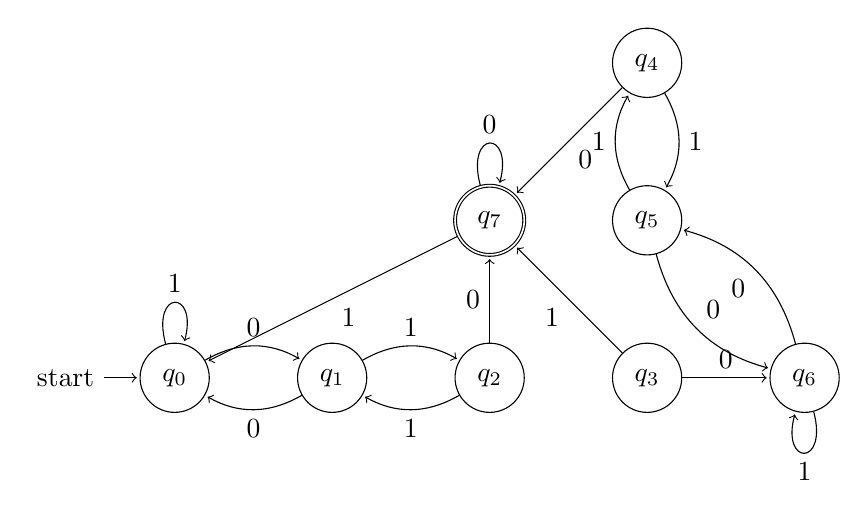
\begin{tikzpicture}[shorten >=1pt,node distance=2cm,on grid,auto]
  \node[state,initial] (q0) {$q_0$};
  \node[state] (q1) [right = of q0] {$q_1$};
  \node[state] (q2) [right = of q1] {$q_2$};
  \node[state] (q3) [right = of q2] {$q_3$};
  \node[state] (q5) [above = of q3] {$q_5$};
  \node[state] (q4) [above = of q5]{$q_4$};
  \node[state] (q6) [right = of q3] {$q_6$};
  \node[state,accepting] (q7) [above = of q2] {$q_7$};
  \path[->]
  (q0)
  edge [bend left] node [] {$0$} (q1)
  edge [loop above] node [] {$1$} ()
  (q1)
  edge [bend left] node [] {$0$} (q0)
  edge [bend left] node [] {$1$} (q2)
  (q2)
  edge [] node [] {$0$} (q7)
  edge [bend left] node [] {$1$} (q1)
  (q3)
  edge [] node [] {$0$} (q6)
  edge [] node [] {$1$} (q7)
  (q4)
  edge [] node [] {$0$} (q7)
  edge [bend left] node [] {$1$} (q5)
  (q5)
  edge [bend right] node [] {$0$} (q6)
  edge [bend left] node [] {$1$} (q4)
  (q6)
  edge [bend right] node [] {$0$} (q5)
  edge [loop below] node [] {$1$} ()
  (q7)
  edge [loop above] node [] {$0$} ()
  edge [] node [] {$1$} (q0)
  ;
\end{tikzpicture}
\end{center}

\begin{table}[h]
\centering
\begin{tabular}{|l|l|llllll}
\cline{1-2}
$q_1$ & $\times$ &                               &                               &                               &                               &                               &                               \\ \cline{1-3}
$q_2$ & $\times$ & \multicolumn{1}{l|}{$\times$} &                               &                               &                               &                               &                               \\ \cline{1-4}
$q_3$ & $\times$ & \multicolumn{1}{l|}{$\times$} & \multicolumn{1}{l|}{$\times$} &                               &                               &                               &                               \\ \cline{1-5}
$q_4$ & $\times$ & \multicolumn{1}{l|}{$\times$} & \multicolumn{1}{l|}{}         & \multicolumn{1}{l|}{$\times$} &                               &                               &                               \\ \cline{1-6}
$q_5$ & $\times$ & \multicolumn{1}{l|}{}         & \multicolumn{1}{l|}{$\times$} & \multicolumn{1}{l|}{$\times$} & \multicolumn{1}{l|}{$\times$} &                               &                               \\ \cline{1-7}
$q_6$ &          & \multicolumn{1}{l|}{$\times$} & \multicolumn{1}{l|}{$\times$} & \multicolumn{1}{l|}{$\times$} & \multicolumn{1}{l|}{$\times$} & \multicolumn{1}{l|}{$\times$} &                               \\ \hline
$q_7$ & $\times$ & \multicolumn{1}{l|}{$\times$} & \multicolumn{1}{l|}{$\times$} & \multicolumn{1}{l|}{$\times$} & \multicolumn{1}{l|}{$\times$} & \multicolumn{1}{l|}{$\times$} & \multicolumn{1}{l|}{$\times$} \\ \hline
      & $q_0$    & \multicolumn{1}{l|}{$q_1$}    & \multicolumn{1}{l|}{$q_2$}    & \multicolumn{1}{l|}{$q_3$}    & \multicolumn{1}{l|}{$q_4$}    & \multicolumn{1}{l|}{$q_5$}    & \multicolumn{1}{l|}{$q_6$}    \\ \hline
\end{tabular}
\end{table}

We can also remove $q_3$, which cannot be reach from any state.

\begin{center}
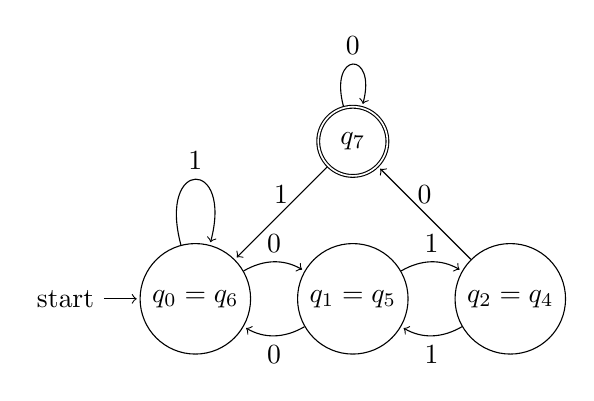
\begin{tikzpicture}[shorten >=1pt,node distance=2cm,on grid,auto]
  \node[state,initial] (q0) {$q_0 = q_6$};
  \node[state] (q1) [right = of q0] {$q_1 = q_5$};
  \node[state] (q2) [right = of q1] {$q_2 = q_4$};
  \node[state,accepting] (q7) [above = of q1] {$q_7$};
  \path[->]
  (q0)
  edge [bend left] node [] {$0$} (q1)
  edge [loop above] node [] {$1$} ()
  (q1)
  edge [bend left] node [] {$0$} (q0)
  edge [bend left] node [] {$1$} (q2)
  (q2)
  edge [] node [above] {$0$} (q7)
  edge [bend left] node [] {$1$} (q1)
  (q7)
  edge [loop above] node [] {$0$} ()
  edge [] node [above] {$1$} (q0)
  ;
\end{tikzpicture}
\end{center}

\end{document}
